\documentclass[11pt]{article}
\usepackage{amsmath,amssymb,graphicx}
\usepackage[letterpaper ,left=2cm,top=2.25cm,bottom=2.25cm,right=2.5cm,nohead,nofoot]{geometry}
\usepackage{color}
\usepackage{bm}
\usepackage{bbold}
\renewcommand{\vec}[1]{\mathbf{#1}}
\DeclareMathOperator{\sgn}{sgn}
\pagestyle{empty}
\usepackage[T1]{fontenc}
%\usepackage{times}
\IfFileExists{newtxtext.sty}
   {\usepackage{newtxtext,newtxmath}}
   {\IfFileExists{stix.sty}
      {\usepackage{stix}}
      {\IfFileExists{mathptmx.sty}
      {\usepackage{mathptmx}}{} } }
\usepackage[scaled]{beramono}
\begin{document}

\begin{center}
{\large\bf Physics 540: Class 16}\\
   {\small Thursday, June 22, 2021}

\end{center}

We want to simulate two balls with masses $m_1$, $m_2$ and radii $R_1$, $R_2$ under freefall conditions:
\begin{alignat*}{2} x_i(t) &= x_i(0) + \varv_{i,x}(0)t, \ \ \ & y_i(t) &= y_i(0) + \varv_{i,y}(0)t - \frac{1}{2}gt^2,\\
\varv_{x,i}(t) &= \varv_{x,i}(0), &\varv_{y,i}(t) &= \varv_{y,i}(0) - gt.
\end{alignat*}
We make the approximation that motion is confined to a common plane. Alternatively, you might imagine that we're actually simulating discs on an air hockey table that's not quite level.

The positions and velocities are updated in the function \verb!advance! according to the formulae above. Those data are organized in a \verb!Ball! structure that is passed by  reference. At each time step $\Delta t \leftrightarrow $~\verb!dt!, we 
solve the quadratic equation $(x_2-x_1)^2 + (y_2-y_1)^2 = (R_1+R_2)^2$
for the possible collision times $t_{c1}$ and $t_{c2}$. (A complex-conjugated pair lying off the real axis indicates that there is no collision).
We take the actual collision time to be the smallest such time that lies in the future ($t_c > 0$).

\begin{center}
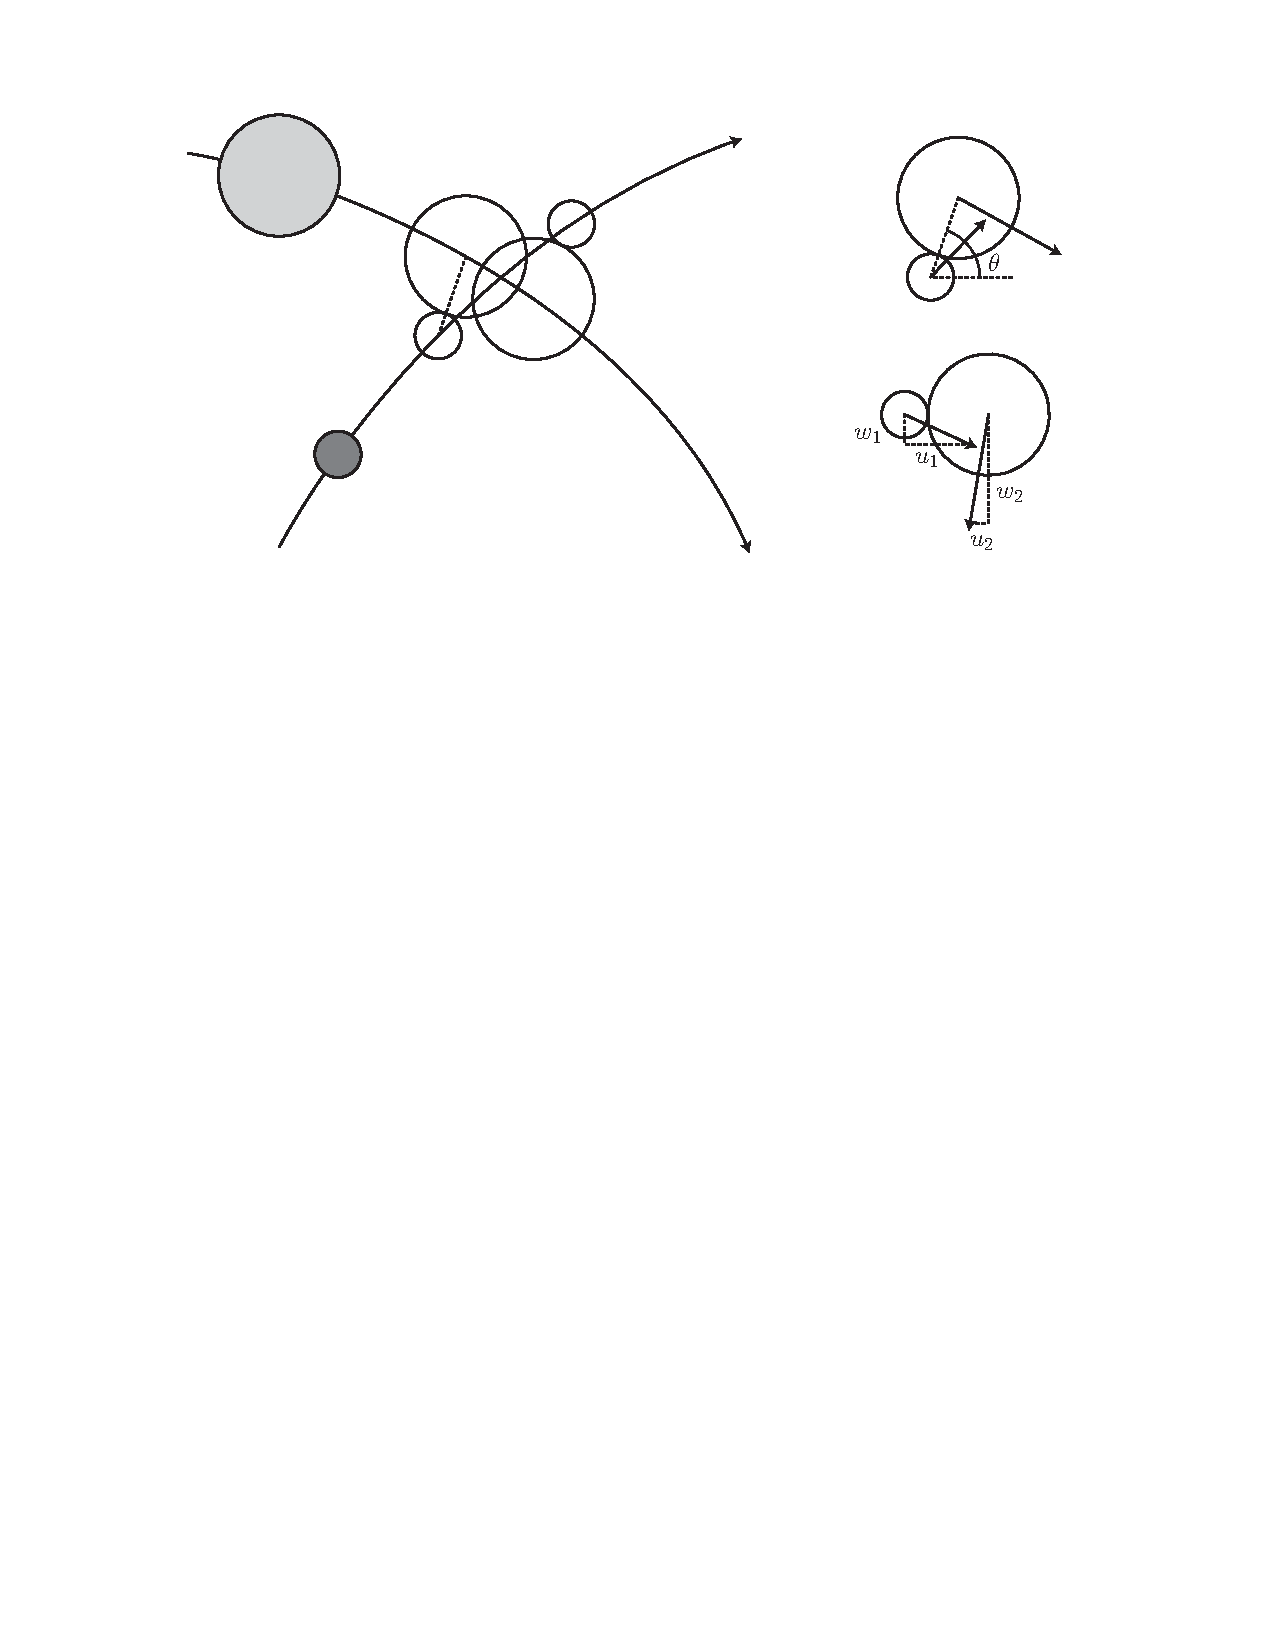
\includegraphics[scale=0.8]{collision.pdf}
\end{center}

If the collision lies more than $\Delta t$ in the future, then we simply advance the particles to their $t+\Delta t$ positions.
If $0 < t_c < \Delta t$, however, we evolve by $t_c$, recompute the velocities after collision (by calling 
\verb!elastic_scatter!) and then evolve by $\Delta t - t_c$.
The new velocities can easy be determined by rotating to a reference frame in which the particles
collide head-on along one of the orthogonal axes:
\[ \begin{pmatrix}
u_i \\
w_i
\end{pmatrix}
= \begin{pmatrix}
\cos \theta & \sin \theta\\
-\sin \theta & \cos \theta
\end{pmatrix}
\begin{pmatrix}
\varv_{i,x}\\
\varv_{i,y}
\end{pmatrix}.
\]
The velocities $u_1$ and $u_2$ take new values
\begin{align*}
 u_1' &= \frac{u_1(m_1-m_2)+2m_2u_2}{m_1+m_2}\\
 u_2' &= \frac{u_2(m_2-m_1)+2m_1u_1}{m_1+m_2}
\end{align*}
and are rotated back to the conventional frame:
\[\begin{pmatrix}
\varv_{i,x}'\\
\varv_{i,y}'
\end{pmatrix}
= \begin{pmatrix}
\cos \theta & -\sin \theta\\
\sin \theta & \cos \theta
\end{pmatrix}
\begin{pmatrix}
u_i' \\
w_i
\end{pmatrix}.
\]

On the other hand, if the balls are perfectly sticky and weld to one another on collision, the final velocities of both balls must be identical. Conservation of momentum tells us that
\begin{align*}
\varv'_{1,x} &= \varv'_{2,x} = \frac{m_1\varv_{1,x} + m_2\varv_{2,x}}{m_1+m_2},\\
\varv'_{1,y} &= \varv'_{2,y} = \frac{m_1\varv_{1,y} + m_2\varv_{2,y}}{m_1+m_2}.
\end{align*}
We can implement this in the function \verb!inelastic_scatter!
and just comment out the \verb!elastic_scatter! function we were
using previously:
\small\begin{verbatim}
inelastic_scatter();
//elastic_scatter();
\end{verbatim}
Here, it's good to check what happens to the conservation of energy.

\end{document}
